
%% This is an example first chapter.  You should put chapter/appendix that you
%% write into a separate file, and add a line \include{yourfilename} to
%% main.tex, where `yourfilename.tex' is the name of the chapter/appendix file.
%% You can process specific files by typing their names in at the 
%% \files=
%% prompt when you run the file main.tex through LaTeX.
\section{Stability}

\subsection{Laminar to Turblent Transition}

The low Reynold number of paper airplane aerodynamics contributes a lot towards the
stability of the flight.
The Reynold number of paper airplane flight is on the order of $10^4$.
Therefore, variations of airfoil characteristics will result in rapid changes in 
the stability. At low Reynold numbers, the laminar boundary layer has great 
influence. There is a big difference between turbulent flow and laminar boundary
layers. Laminar boundary layer doesn't respond well to an increasing
pressure gradient in the direction of flow, whereas turbulent flow does.
However, turbulent flow results in large frictional effects.

One aspect of the laminar boundary layer is the location in which it separates from the surface.
When the laminar boundary layer seperates from the surface, this results Kelvin
Helmholtz instability, vortices, and finally a turbulent boundary layer. 
Because of the instability this transition between turbulence and laminar flow 
can cause, predicting this location is important in the stability of the flight.
This transition location also results in hysterisis effects. Before separation
occurs, increasing angle of attack will increase lift. But afterwards,
decreasing the angle of attack does not return to the same lift. This effect is
illustrated in figure~\ref{fig:boundary_layer_transition}.

\begin{figure}[hl]
  \centering
    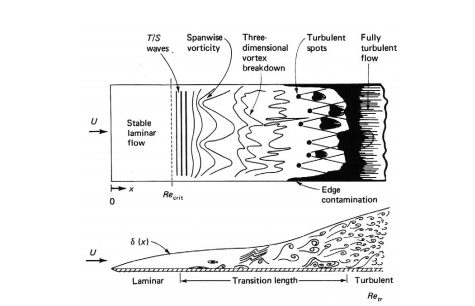
\includegraphics[scale=.5]{figures/boundary_layer_transition.png}
    \caption{Illustration of the boundary layer process}
  \label{fig:boundary_layer_transition}
\end{figure}



\begin{enumerate}
\item For Reynold numbers between 1000 and 10000 the boundary layer flow is laminar
and doesn't transition into trubulent flow. This type of flight is seen with
the dragon fly and the house fly. 
\item  For Reynold numbers between 10000 and 30000 the boundary layer is laminar but
it can separate. When it separates it does not reattach.
\item At 30000 to 70000 there are hysterisis effects because of the transition. 

\end{enumerate}

\subsection{Lateral Stability}

\subsubsection{Lateral Forces}

To analyze the lateral stability, we first must know about the lateral forces on the wings.
For a paper airplane, we can model the wings as a inifinte flat plate. Since it is
an infinite flat plate, we can analyze it with a complex potential in two dimensions.
By means of conformal mapping, we can collapse a cylinder to a flat plate by

\[Z = z + \frac{a^2}{z}\].

\begin{figure}[hl]
  \centering
    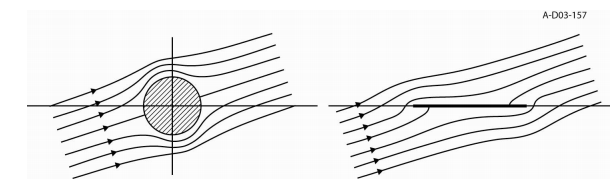
\includegraphics[scale=.5]{figures/flatplate1.png}
    \caption{Dihedral vs Anhedral wings}
  \label{fig:dihedraleffect}
\end{figure}

Now let us consider a flow at an angle $\alpha$. A cylinder with a radius $r$
would result in a potential
\[w(z) = Ue^{i\alpha}(z + \frac{a^2}{z}) \]
After the conformal transformation, we see that the velocity now becomes
\[u - iv = \od{W}{Z} = \frac{\od{w}{z}}{\od{Z}{z}} = \frac{Ue^{-i\alpha}-Ue^{i\alpha}\frac{a^2}{z^2}
- \frac{i \Gamma}{2\pi z}}{1 - \frac{a^2}{z^2}}\]

In order to choose $\Gamma$ we must use the fact that the singularity at the trailing edge, 
$Z=2a$ or $z=a$ must be removed, from the condition. This condition occurs because 
a boundary layer prevents the flow from turning the sharp corner at the trailing edge.
The physical solution from complex flow theory depends on frictional forces.

Therefore we can find the circulation.

\[ \Gamma = -4\pi Ua \sin(\alpha) \]

This allows us to find the lift by the Kutta-Joukowski theorem.

\[L = \rho U \Gamma\]
\begin{equation}
\label{eq:flat_plat_cl}
C_L = 2\pi sin(\alpha)
\end{equation}

\subsection{Dihedral vs Anhedral}

Dihedral and anhedral refer to the angle between the wings and the horizontal plane.
Dihedral wings means that the wings point upwards, and the anhedral wings means the wings point
downwards as shown in Figure~\ref{fig:dihedraleffect}. Dihedral wings have more lateral 
stability than anhedral wings.

\begin{figure}[hl]
  \centering
    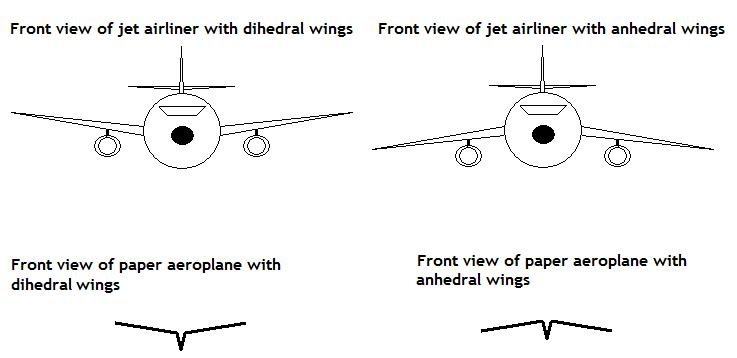
\includegraphics[scale=.5]{figures/dihedraleffect.png}
    \caption{Dihedral vs Anhedral wings}
  \label{fig:dihedraleffect}
\end{figure}

The bank angle is defined as the angle about the axis along
the plane's motion. Let us call the bank angle $\phi$. When the aircraft is
banked, this results in a rolling moment, called the dihedral effect. If the
rolling moment opposes the bank, the dihedral effect is positive. In order for
there to be stability, the dihedral effect needs to be positive. There are many
different factors that can contribute to the dihedral effect: the shape of the wings,
the wing placement, tail height, etc. 

To analyze this effect in more detail we will show that a dihedral aircraft has 
a positive dihedral effect. When the aircraft is banked we see that there is a net force
to the side, this is called sideslip (Figure~\ref{fig:dihedral1}). 
However we see that the forces on the wings do not 
contribute to the dihedral effect yet.


\begin{figure}[hl]
  \centering
    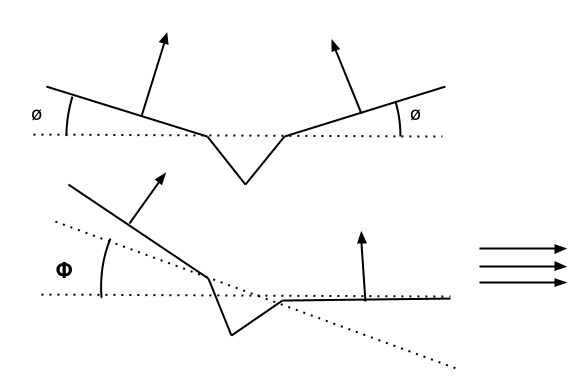
\includegraphics[scale=.5]{figures/dihedral1.png}
    \caption{SideSlip}
  \label{fig:dihedral1}
\end{figure}

At this point, with respect to the plane's frame of reference, there is air flowing 
to the side that will contribute to a dihedral effect. However, we see that for the
corresponding anhedral plane, the bottom wing would be affected more by the air, causing
a negative dihedral effect (Figure~\ref{fig:dihedral2}). If the bank angle is $\phi$ and
the angle that the wings make with the horizontal is $\theta$ then after factoring in
the banked angle, the right wing has an angle of attack of  $\theta - \phi$.
The left wing has an angle of attack $- \theta - \phi$.

\begin{figure}[hl]
  \centering
    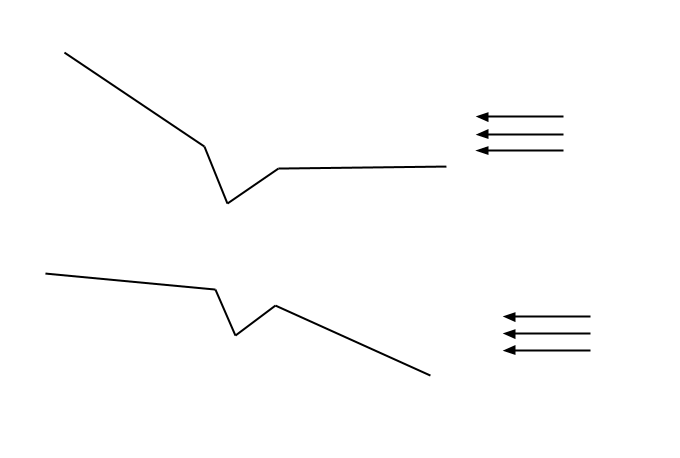
\includegraphics[scale=.5]{figures/dihedral2.png}
    \caption{Positive vs Negative dihedral effect}
  \label{fig:dihedral2}
\end{figure}

If we assume that the wings are approximate flat plates, we can say that the
coefficient of lift is approximately $2\pi\sin(\alpha)$ as shown in Equation~\ref{flat_plate_cl}. 
$\alpha$ is
the angle of attack and $\beta$ is a constant. For small angles it is 
approximately $2\pi(\alpha)$. So the left wing will exerience a downward force
and the right wing will experience an upwards force, straightning the plane out.




